\documentclass[14pt]{extbook}
\usepackage{multicol, enumerate, enumitem, hyperref, color, soul, setspace, parskip, fancyhdr} %General Packages
\usepackage{amssymb, amsthm, amsmath, latexsym, units, mathtools} %Math Packages
\everymath{\displaystyle} %All math in Display Style
% Packages with additional options
\usepackage[headsep=0.5cm,headheight=12pt, left=1 in,right= 1 in,top= 1 in,bottom= 1 in]{geometry}
\usepackage[usenames,dvipsnames]{xcolor}
\usepackage{dashrule}  % Package to use the command below to create lines between items
\newcommand{\litem}[1]{\item#1\hspace*{-1cm}\rule{\textwidth}{0.4pt}}
\pagestyle{fancy}
\lhead{Progress Quiz 4}
\chead{}
\rhead{Version A}
\lfoot{5346-5907}
\cfoot{}
\rfoot{Summer C 2021}
\begin{document}

\begin{enumerate}
\litem{
Choose the equation of the function graphed below.
\begin{center}
    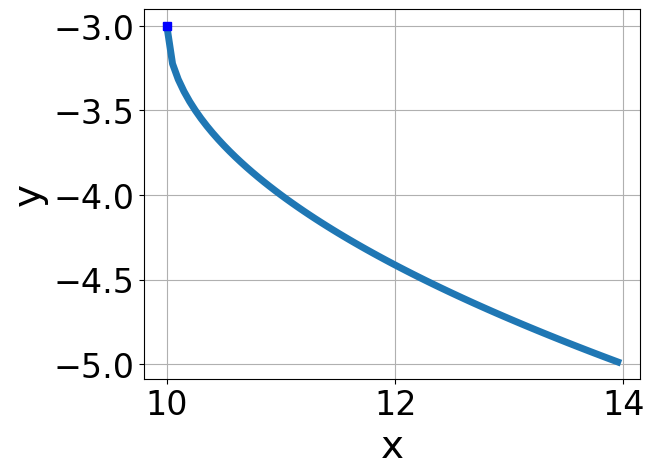
\includegraphics[width=0.5\textwidth]{../Figures/radicalGraphToEquationA.png}
\end{center}
\begin{enumerate}[label=\Alph*.]
\item \( f(x) = - \sqrt{x + 10} - 3 \)
\item \( f(x) = \sqrt{x + 10} - 3 \)
\item \( f(x) = - \sqrt{x - 10} - 3 \)
\item \( f(x) = \sqrt{x - 10} - 3 \)
\item \( \text{None of the above} \)

\end{enumerate} }
\litem{
Choose the graph of the equation below.\[ f(x) = \sqrt[3]{x - 6} + 4 \]\begin{enumerate}[label=\Alph*.]
\begin{multicols}{2}\item 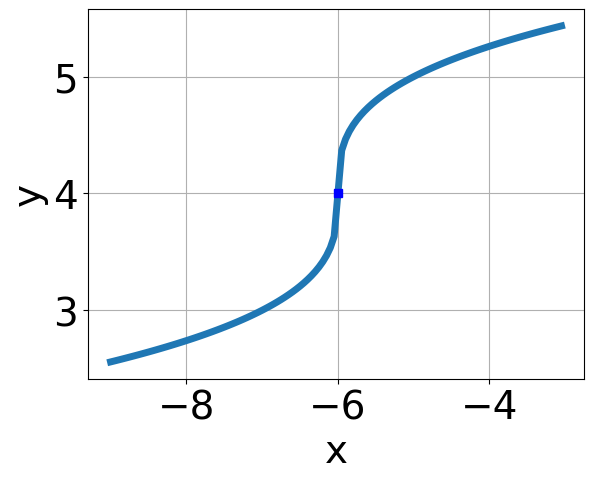
\includegraphics[width = 0.3\textwidth]{../Figures/radicalEquationToGraphCopyAA.png}\item 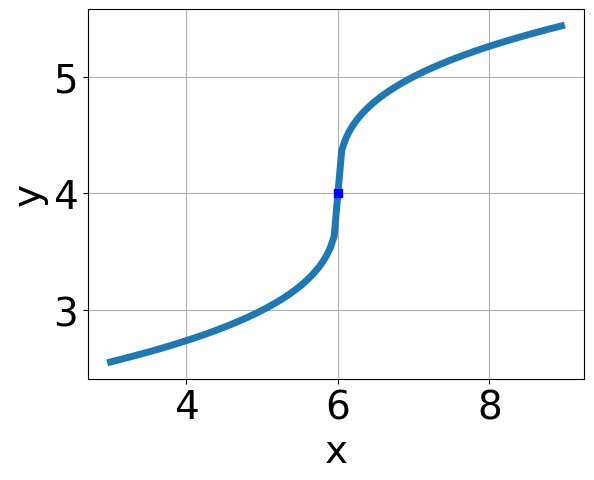
\includegraphics[width = 0.3\textwidth]{../Figures/radicalEquationToGraphCopyBA.png}\item 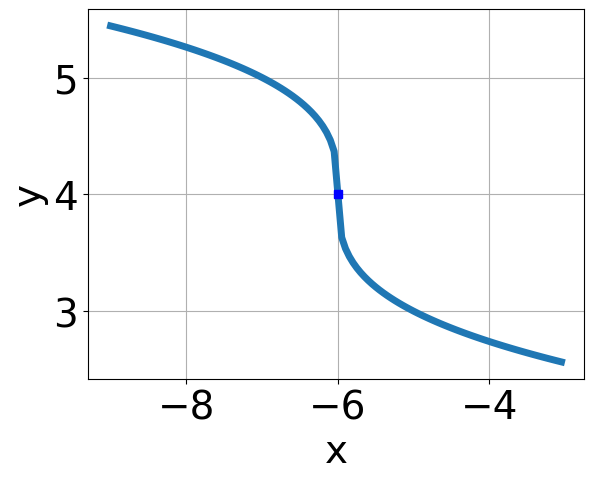
\includegraphics[width = 0.3\textwidth]{../Figures/radicalEquationToGraphCopyCA.png}\item 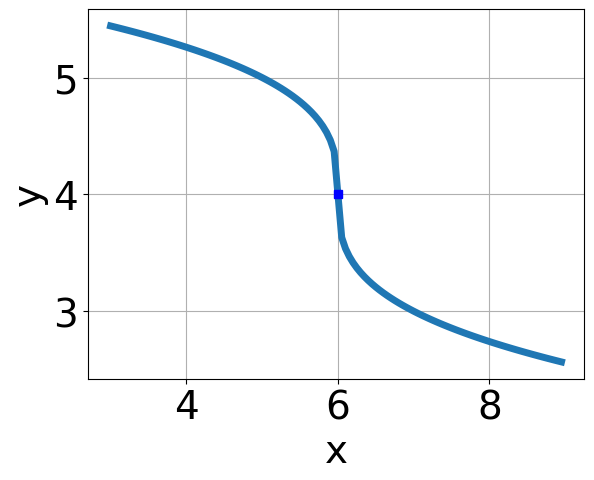
\includegraphics[width = 0.3\textwidth]{../Figures/radicalEquationToGraphCopyDA.png}\end{multicols}\item None of the above.
\end{enumerate} }
\litem{
Choose the graph of the equation below.\[ f(x) = \sqrt{x + 10} + 3 \]\begin{enumerate}[label=\Alph*.]
\begin{multicols}{2}\item 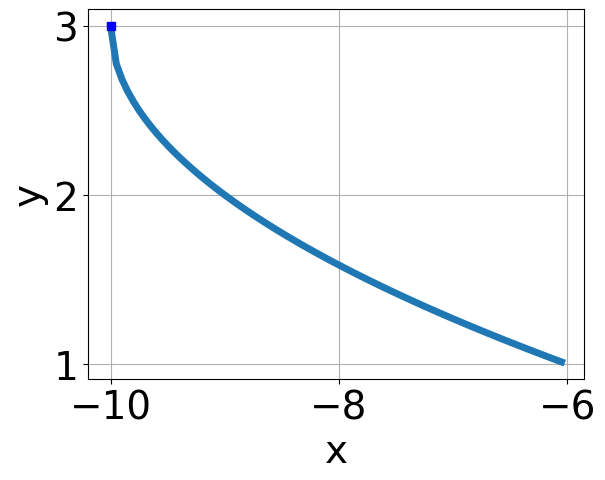
\includegraphics[width = 0.3\textwidth]{../Figures/radicalEquationToGraphAA.png}\item 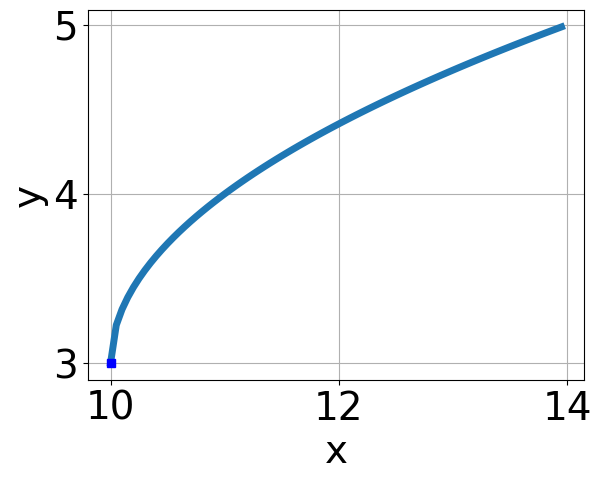
\includegraphics[width = 0.3\textwidth]{../Figures/radicalEquationToGraphBA.png}\item 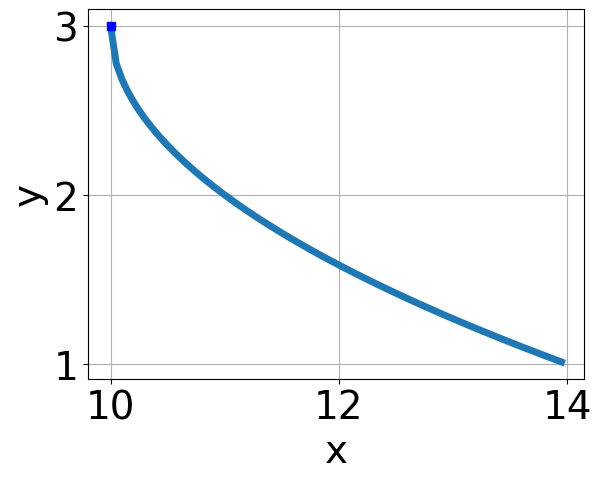
\includegraphics[width = 0.3\textwidth]{../Figures/radicalEquationToGraphCA.png}\item 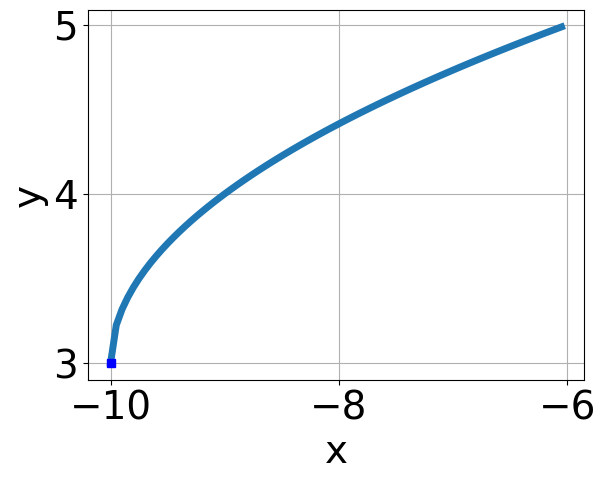
\includegraphics[width = 0.3\textwidth]{../Figures/radicalEquationToGraphDA.png}\end{multicols}\item None of the above.
\end{enumerate} }
\litem{
Solve the radical equation below. Then, choose the interval(s) that the solution(s) belongs to.\[ \sqrt{48 x^2 - 30} - \sqrt{-4 x} = 0 \]\begin{enumerate}[label=\Alph*.]
\item \( x \in [-2.83,0.17] \)
\item \( x \in [-0.25,3.75] \)
\item \( \text{All solutions lead to invalid or complex values in the equation.} \)
\item \( x_1 \in [-0.25, 3.75] \text{ and } x_2 \in [0.79,0.87] \)
\item \( x_1 \in [-2.83, 0.17] \text{ and } x_2 \in [0.67,0.76] \)

\end{enumerate} }
\litem{
Solve the radical equation below. Then, choose the interval(s) that the solution(s) belongs to.\[ \sqrt{9 x + 5} - \sqrt{5 x + 5} = 0 \]\begin{enumerate}[label=\Alph*.]
\item \( x \in [-2.98,-1.79] \)
\item \( x_1 \in [-1.09, -0.92] \text{ and } x_2 \in [-0.87,-0.55] \)
\item \( x_1 \in [-0.63, -0.24] \text{ and } x_2 \in [-0.55,0.11] \)
\item \( x \in [-0.45,0.4] \)
\item \( \text{All solutions lead to invalid or complex values in the equation.} \)

\end{enumerate} }
\litem{
Choose the equation of the function graphed below.
\begin{center}
    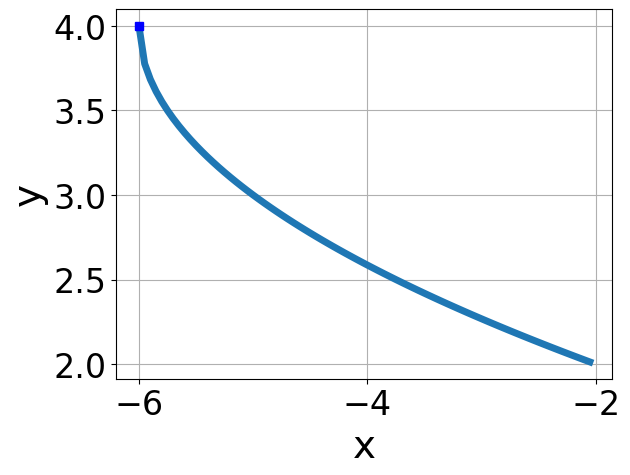
\includegraphics[width=0.5\textwidth]{../Figures/radicalGraphToEquationCopyA.png}
\end{center}
\begin{enumerate}[label=\Alph*.]
\item \( f(x) = - \sqrt{x + 6} + 4 \)
\item \( f(x) = \sqrt{x - 6} + 4 \)
\item \( f(x) = \sqrt{x + 6} + 4 \)
\item \( f(x) = - \sqrt{x - 6} + 4 \)
\item \( \text{None of the above} \)

\end{enumerate} }
\litem{
Solve the radical equation below. Then, choose the interval(s) that the solution(s) belongs to.\[ \sqrt{-24 x^2 + 21} - \sqrt{10 x} = 0 \]\begin{enumerate}[label=\Alph*.]
\item \( \text{All solutions lead to invalid or complex values in the equation.} \)
\item \( x \in [-1.29,-0.35] \)
\item \( x_1 \in [-1.29, -0.35] \text{ and } x_2 \in [0.64,0.94] \)
\item \( x_1 \in [0.44, 1.41] \text{ and } x_2 \in [0.96,1.3] \)
\item \( x \in [0.44,1.41] \)

\end{enumerate} }
\litem{
Solve the radical equation below. Then, choose the interval(s) that the solution(s) belongs to.\[ \sqrt{-3 x + 2} - \sqrt{-6 x + 7} = 0 \]\begin{enumerate}[label=\Alph*.]
\item \( \text{All solutions lead to invalid or complex values in the equation.} \)
\item \( x \in [1.08,1.84] \)
\item \( x_1 \in [-0.34, 0.84] \text{ and } x_2 \in [1.4,2] \)
\item \( x \in [-3.15,-1.87] \)
\item \( x_1 \in [-0.34, 0.84] \text{ and } x_2 \in [0.2,1.6] \)

\end{enumerate} }
\litem{
What is the domain of the function below?\[ f(x) = \sqrt[3]{-4 x + 9} \]\begin{enumerate}[label=\Alph*.]
\item \( \text{The domain is } (-\infty, a], \text{   where } a \in [-2.6, 0.5] \)
\item \( \text{The domain is } (-\infty, a], \text{   where } a \in [1.3, 2.8] \)
\item \( \text{The domain is } [a, \infty), \text{   where } a \in [1.2, 2.7] \)
\item \( (-\infty, \infty) \)
\item \( \text{The domain is } [a, \infty), \text{   where } a \in [-1.4, 1.6] \)

\end{enumerate} }
\litem{
What is the domain of the function below?\[ f(x) = \sqrt[4]{7 x + 3} \]\begin{enumerate}[label=\Alph*.]
\item \( [a, \infty), \text{ where } a \in [-2.2, 1.3] \)
\item \( (-\infty, \infty) \)
\item \( (-\infty, a], \text{where } a \in [-3.5, -0.5] \)
\item \( [a, \infty), \text{where } a \in [-5.8, -2.2] \)
\item \( (-\infty, a], \text{where } a \in [-1.6, 0.1] \)

\end{enumerate} }
\end{enumerate}

\end{document}